%%%%%%%%%%%%%%
%	GROUPVIEW
%%%%%%%%%%%%%%%%
\subsubsection{GroupView (class)}
\label{spegroV}
\begin{figure}[!h]
\centering
			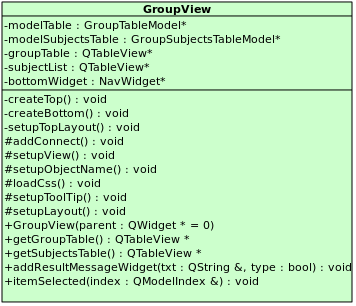
\includegraphics[width=0.5\linewidth]{./Content/Immagini/view/GroupView.png}
			\caption{Diagramma Classe GroupView: attributi e metodi}
			\label{cl_groview}
\end{figure}
\paragraph{Descrizione \\}
Classe che rappresenta il widget per la visualizzazione di tutti i gruppi di \subject{} presenti all'interno di \project.
\paragraph{Utilizzo\\}
La classe implementerà i metodi virtuali puri della superclasse inoltre darà la possibilità all'utente di visualizzare l'elenco di tutti i gruppi di \subject{} fino a quel momento creati e memorizzati dentro a \project. Selezionando un gruppo, sarà possibile visualizzare le informazioni relative a quel gruppo, come per esempio i \subject{} contenuti al suo interno.
\paragraph{Classi ereditate\\}
\begin{itemize}
\item Window::APanel.
\end{itemize}
%%%%%%%ATTRIBUTI%%%%%%%%%%%
\paragraph{\textcolor{black}{Attributi\\}}
\begin{itemize}
\item\color{teal}\verb!-modelTable: GroupTableModel *!
\color{black}
\subparagraph{Descrizione:}
Modello che contiene i gruppi di\subject{} presenti nel sistema fino a quel momento.

%modelSub
\item\color{teal}\verb!-modeSubjectslTable: GroupSubjectsTableModel *!
\color{black}
\subparagraph{Descrizione:}
Modello che contiene i \subject{} presenti in un determinato gruppo di \subject{} fino a quel momento presenti nel sistema.

%tabelView
\item\color{teal}\verb!-groupTable: QTabelView*!
\color{black}
\subparagraph{Descrizione:}
Contiene la lista dei gruppi di \subject{} contenuti nel campo dati \emph{modelTable}.

%tabelView
\item\color{teal}\verb!-subjectList: QTabelView*!
\color{black}
\subparagraph{Descrizione:}
Contiene la lista dei \subject{} contenuti nel campo dati \emph{modelSubjectsTable}.

%bottomWidget
\item\color{teal}\verb! bottomWidget:NavWidget*!
\color{black} 
\subparagraph{Descrizione:}
Puntatore al widget che rappresenta la parte bassa della finestra contentente i pulsanti per tornare indietro, la visualizzazione della guida interattiva, la possibilità di editare un gruppo e salvare successivamente le modifiche.
\end{itemize}
%%%%%%%%%  METODI
\paragraph{\textcolor{black}{Metodi\\}}
\begin{itemize}
%costruttore
\item\color{blue}\verb! + GroupView(parent : QWidget*=0)!
\color{black}
\subparagraph{Descrizione:}Costruttore per la classe GroupView. 
\subparagraph{Argomenti:}
\begin{itemize}
\item \color{RoyalPurple}\verb!parent: QWidget*=0!  \\ Puntatore al QWidget padre di GroupView.
\end{itemize}

%setupLayout()
\item\color{blue}\verb! #setupLayout():void!
\color{black}
\subparagraph{Descrizione:}Metodo che implementa il contratto fornito dalla classe astratta \hyperref[speAPanel]{APanel}.
\subparagraph{Note:}
\begin{itemize}
\item questo metodo deve essere marcato virtuale;
\item questo metodo è stato ridefinito.
\end{itemize}
 
%createTop
\item\color{blue}\verb! -createTop():void!
\color{black}
\subparagraph{Descrizione:}Metodo che ha il compito di costruire la parte in alto del widget contenente l'elenco dei \subject e a lato lo spazio per visualizzare le informazioni.
 
%createButtom
\item\color{blue}\verb! -createButtom():void!
\color{black}
\subparagraph{Descrizione:}Metodo che ha il compito di costruire la parte in basso del widget contenente il pulsante per ritornare alla pagine iniziale, e per l'accesso alla guida.

%setupTopLayout
\item\color{blue}\verb! -setupTopLayout():void!
\color{black}
\subparagraph{Descrizione:} Metodo che ha il compito di impostare la parte alta del layout della finestra.
  
%LOADCSS
\item\color{blue}\verb! #loadCss():void!
\color{black}
\subparagraph{Descrizione:} Metodo che implementa il contratto fornito dalla classe astratta \hyperref[speAPanel]{APanel}.
 \subparagraph{Note}
 \begin{itemize}
  \item questo metododeve essere marcato virtuale;
 \item questo metodo è stato ridefinito.
 \end{itemize}
 
%setupObjectName
\item\color{blue}\verb! #setupObjectName():void!
\color{black}
\subparagraph{Descrizione:}Metodo che implementa il contratto fornito dalla classe astratta \hyperref[speAPanel]{APanel}.
 \subparagraph{Note}
 \begin{itemize}
  \item questo deve essere marcato virtuale;
 \item questo metodo è stato ridefinito.
 \end{itemize}
 
%setupToolTip
\item\color{blue}\verb! #setupToolTip():void!
\color{black}
\subparagraph{Descrizione:}Metodo che implementa il contratto fornito dalla classe astratta \hyperref[speAPanel]{APanel}.
 \subparagraph{Note}
 \begin{itemize}
 \item questo metodo deve essere marcato virtuale;
 \item questo metodo è stato ridefinito.
 \end{itemize}
 
%addConnect
\item\color{blue}\verb! #addConnect():void!
\color{black}
\subparagraph{Descrizione:}Metodo che implementa il contratto fornito dalla classe astratta \hyperref[speAPanel]{APanel}.
 \subparagraph{Note}
 \begin{itemize}
 \item questo metodo deve essere marcato costante;
 \item questo metodo deve essere marcato virtuale;
 \item questo metodo è stato ridefinito.
 \end{itemize}
 
%setupView
\item\color{blue}\verb! #setupView():void!
\color{black}
\subparagraph{Descrizione:}Metodo che implementa il contratto fornito dalla classe astratta \hyperref[speAPanel]{APanel}.
 \subparagraph{Note}
 \begin{itemize}
 \item questo metodo deve essere marcato virtuale;
 \item questo metodo è stato ridefinito.
 \end{itemize}

%getGroup
\item\color{blue}\verb! +getGroupTable():QTabelView*!
\color{black}
\subparagraph{Descrizione:}Metodo che ritorna il puntatore al campo dati \emph{groupTable}.
 \subparagraph{Note}
 \begin{itemize}
 \item questo metodo deve essere marcato costante.
 \end{itemize}

%getsubje
\item\color{blue}\verb! +getSubjectsTable():QTabelView*!
\color{black}
\subparagraph{Descrizione:}Metodo che ritorna il puntatore al campo dati \emph{modelSubjectTable}.
 \subparagraph{Note}
 \begin{itemize}
 \item questo metodo deve essere marcato costante.
 \end{itemize}
%addResultMessag
\item \color{blue} \verb! + addResultMessageWidget(txt: const QString&, type: bool):void! 
\color{black}
\subparagraph{Descrizione:} Metodo che ha il compito di aggiungere il messaggio di risultato per avvenuta operazione o meno a seconda del valore del secondo parametro passato.
\subparagraph{Argomenti:}
\begin{itemize}
\item \color{RoyalPurple} \verb! txt: const QString& ! \\Rappresenta il testo da mostrare all'utente all'interno del widget;
\item \color{RoyalPurple} \verb!type : bool ! \\ Vale true se il messaggio è un messaggio di successo, false se il messaggio è di errore.
\end{itemize}
\subparagraph{Note:}
\begin{itemize}
\item il metodo deve essere marcato virtuale.
\end{itemize}

%itemSelected
\item\color{blue}\verb! +itemSelected(index:QModelIndex&): void! (signal)
\color{black} 
\subparagraph{Descrizione:}
Signal\g{} emesso quando l'utente seleziona un elemento da una tabella, che sia quella contentente la lista di gruppi di \subject{} o quella con la lista dei \subject{} per un determinato gruppo.
\subparagraph{Attributi:}
\begin{itemize}
\item \color{RoyalPurple}\verb! index: QModelIndex& ! \\ rappresenta l'indice della tabella selezionato.
\end{itemize}
\end{itemize}
\pagebreak
\color{black}
%%%%%%%%%%%%%%%%%%%%%%
% PROTOCOLSVIEW
%%%%%%%%%%%%%%%%%%%%%
\subsubsection{ProtocolsView (class)}
\label{speproV}
\begin{figure}[!h]
\centering
			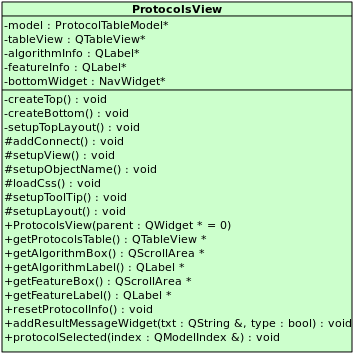
\includegraphics[width=0.5\linewidth]{./Content/Immagini/view/ProtocolsView.png}
			\caption{Diagramma Classe ProtocolsView: attributi e metodi}
			\label{cl_proview}
\end{figure}
\paragraph{Descrizione \\}
Classe che rappresenta il widget per la visualizzazione di tutti i \protocol{} presenti all'interno di \project.
\paragraph{Utilizzo\\}
La classe implementerà i metodi virtuali puri della superclasse inoltre darà la possibilità all'utente di visualizzare l'elenco di tutti i \protocol{} fino a quel momento creati e memorizzati dentro a \project. Selezionando un \protocol{}, sarà possibile visualizzare le informazioni relative a quel \protocol{}: feature\g{} presenti con il valore dei parametri (qualora fossero presenti), e algoritmo di clustering\g{} con valore dei parametri.
\paragraph{Classi ereditate\\}
\begin{itemize}
\item Window::APanel.
\end{itemize}
%%%%%%%ATTRIBUTI%%%%%%%%%%%
\paragraph{\textcolor{black}{Attributi\\}}
\begin{itemize}
\item\color{teal}\verb!-model: protocolTableModel *!
\color{black}
\subparagraph{Descrizione:}Modello che contiene i \protocol{} presenti nel sistema fino a quel momento.

%tabelView
\item\color{teal}\verb!-tableView: QTabelView*!
\color{black}
\subparagraph{Descrizione:}
Contiene la lista dei \protocol{} contenuti nel campo dati \emph{model}.

%algInfo
\item\color{teal}\verb!-algorithmInfo: QLabel*!
\color{black}
\subparagraph{Descrizione:}
Contiene le informazioni relative all'algoritmo di clustering\g{} del \protocol{} selezionato, qualora fosse presente.

%featInfo
\item\color{teal}\verb!-featureInfo: QLabel*!
\color{black}
\subparagraph{Descrizione:}
Contiene le informazioni relative alle Feature\g{} del \protocol{} selezionato qualora fosse presente almeno una Feature\g{}.

%bottomWidget
\item\color{teal}\verb! bottomWidget:NavWidget*!
\color{black} 
\subparagraph{Descrizione:}
Puntatore al widget che rappresenta la parte bassa della finestra contentente i pulsanti per tornare indietro, la visualizzazione della guida interattiva, la possibilità di eliminare un \protocol{} e confermare l'operazione.
\end{itemize}
%%%%%%%%%  METODI
\paragraph{\textcolor{black}{Metodi\\}}
\begin{itemize}
%costruttore
\item\color{blue}\verb! + ProtocolsView(parent : QWidget*=0)!
\color{black}
\subparagraph{Descrizione:}Costruttore per la classe ProtocolsView. 
\subparagraph{Argomenti:}
\begin{itemize}
\item \color{RoyalPurple}\verb!parent: QWidget*=0  !\\ Puntatore al QWidget padre di ProtocolsView.
\end{itemize}

%setupLayout()
\item\color{blue}\verb! #setupLayout():void!
\color{black}
\subparagraph{Descrizione:}Metodo che implementa il contratto fornito dalla classe astratta \hyperref[speAPanel]{APanel}.
\subparagraph{Note:}
\begin{itemize}
\item questo metodo deve essere marcato virtuale;
\item questo metodo è stato ridefinito.
\end{itemize}
 
%createTop
\item\color{blue}\verb! -createTop():void!
\color{black}
\subparagraph{Descrizione:}Metodo che ha il compito di costruire la parte in alto del widget contenente l'elenco dei \subject e a lato lo spazio per visualizzare le informazioni.
 
%createButtom
\item\color{blue}\verb! -createButtom():void!
\color{black}
\subparagraph{Descrizione:}Metodo che ha il compito di costruire la parte in basso del widget contenente il pulsante per ritornare alla pagine iniziale, e per l'accesso alla guida.

%setupTopLayout
\item\color{blue}\verb! -setupTopLayout():void!
\color{black}
\subparagraph{Descrizione:}Metodo che ha il compito di impostare la parte alta del layout della finestra.
  
%LOADCSS
\item\color{blue}\verb! #loadCss():void!
\color{black}
\subparagraph{Descrizione:}Metodo che implementa il contratto fornito dalla classe astratta \hyperref[speAPanel]{APanel}.
 \subparagraph{Note}
 \begin{itemize}
  \item questo metododeve essere marcato virtuale;
 \item questo metodo è stato ridefinito.
 \end{itemize}
 
%setupObjectName
\item\color{blue}\verb! #setupObjectName():void!
\color{black}
\subparagraph{Descrizione:}Metodo che implementa il contratto fornito dalla classe astratta \hyperref[speAPanel]{APanel}.
 \subparagraph{Note}
 \begin{itemize}
  \item questo deve essere marcato virtuale;
 \item questo metodo è stato ridefinito.
 \end{itemize}
 
%setupToolTip
\item\color{blue}\verb! #setupToolTip():void!
\color{black}
\subparagraph{Descrizione:}Metodo che implementa il contratto fornito dalla classe astratta \hyperref[speAPanel]{APanel}.
 \subparagraph{Note}
 \begin{itemize}
 \item questo metodo deve essere marcato virtuale;
 \item questo metodo è stato ridefinito.
 \end{itemize}
 
%addConnect
\item\color{blue}\verb! #addConnect():void!

\color{black}
\subparagraph{Descrizione:}Metodo che implementa il contratto fornito dalla classe astratta \hyperref[speAPanel]{APanel}.
 \subparagraph{Note}
 \begin{itemize}
 \item questo metodo deve essere marcato costante;
 \item questo metodo deve essere marcato virtuale;
 \item questo metodo è stato ridefinito.
 \end{itemize}
 
%setupView
\item\color{blue}\verb! #setupView():void!
\color{black}
\subparagraph{Descrizione:}Metodo che implementa il contratto fornito dalla classe astratta \hyperref[speAPanel]{APanel}.
 \subparagraph{Note}
 \begin{itemize}
 \item questo metodo deve essere marcato virtuale;
 \item questo metodo è stato ridefinito.
 \end{itemize}

%getProtocol
\item\color{blue}\verb! +getProtoclsTable():QTabelView*!
\color{black}
\subparagraph{Descrizione:}Metodo che ritorna il puntatore al campo dati \emph{protocolsTable}.
 \subparagraph{Note}
 \begin{itemize}
 \item questo metodo deve essere marcato costante.
 \end{itemize}

%getAlgInfo
\item\color{blue}\verb! +getAlgorithmLabel():QLabel*!
\color{black}
\subparagraph{Descrizione:}Metodo che ritorna la label contenente le informazioni riguardanti l'algoritmo di clustering\g{} presente nel \protocol{}.
 \subparagraph{Note}
 \begin{itemize}
 \item questo metodo deve essere marcato costante.
 \end{itemize}

%getInf
\item\color{blue}\verb! +getFeatureLabel():QLabel*!
\color{black}
\subparagraph{Descrizione:}Metodo che ritorna la label contenente le informazioni riguardanti le Feature\g{} presenti nel \protocol{}.
 \subparagraph{Note}
 \begin{itemize}
 \item questo metodo deve essere marcato costante.
 \end{itemize}

%getalgoBox
\item\color{blue}\verb! +getAlgorithmBox():QScrollArea*!
\color{black}
\subparagraph{Descrizione:}Metodo che ritorna il puntatore al box contentente le informazioni dell'algoritmo.
 \subparagraph{Note}
 \begin{itemize}
 \item questo metodo deve essere marcato costante.
 \end{itemize}
 
%getFeatBox
\item\color{blue}\verb! +getFeaturesBox():QScrollArea*!
\color{black}
\subparagraph{Descrizione:}Metodo che ritorna il puntatore al box contentente le informazioni dei \protocol{}.
 \subparagraph{Note}
 \begin{itemize}
 \item questo metodo deve essere marcato costante.
 \end{itemize} 
 
%addResultMessag
\item \color{blue} \verb! + addResultMessageWidget(txt: const QString&, type: bool):void! 
\color{black}
\subparagraph{Descrizione:} Metodo che ha il compito di aggiungere il messaggio di risultato per avvenuta operazione o meno a seconda del valore del secondo parametro passato.
\subparagraph{Argomenti:}
\begin{itemize}
\item \color{RoyalPurple} \verb! txt: const QString& !  \\Rappresenta il testo da mostrare all'utente all'interno del widget;
\item \color{RoyalPurple} \verb!type : bool ! \\ Vale true se il messaggio è un messaggio di successo, false se il messaggio è di errore.
\end{itemize}
\subparagraph{Note:}
\begin{itemize}
\item il metodo deve essere marcato virtuale.
\end{itemize}

%resetProtocolInfo
\item\color{blue}\verb! + resetProtocolInfo(): void!
\color{black}
\subparagraph{Descrizione:}Metodo che reimposta il box contenente le informazioni.
 \subparagraph{Note}
 \begin{itemize}
 \item questo metodo deve essere marcato costante.
 \end{itemize}

%protSelected
\item\color{blue}\verb! +protocolSelected(index:QModelIndex&):void! (signal)
\color{black} 
\subparagraph{Descrizione:}
Signal\g{} emesso quando l'utente seleziona un elemento da una tabella, che sia quella contentente la lista di gruppi di \subject{} o quella con la lista dei \subject{} per un determinato gruppo.

\end{itemize}
\color{black}
\pagebreak
%%%%%%%%%%%%%%%%%%%%5
%	DATASETSVIEW
%%%%%%%%%%%%%%%%
\subsubsection{DatasetsView (class)}
\label{spedatV}
\begin{figure}[!h]
\centering
			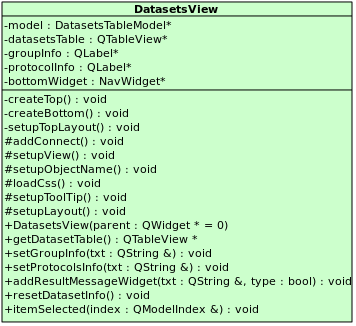
\includegraphics[width=0.5\linewidth]{./Content/Immagini/view/DatasetsView.png}
			\caption{Diagramma Classe DatasetsView: attributi e metodi}
			\label{cl_datview}
\end{figure}
\paragraph{Descrizione \\}
Classe che rappresenta il widget per la visualizzazione di tutti i \dataset{} presenti all'interno di \project.
\paragraph{Utilizzo\\}
La classe implementerà i metodi virtuali puri della superclasse inoltre darà la possibilità all'utente di visualizzare l'elenco di tutti i \dataset{} fino a quel momento creati e memorizzati dentro a \project. Selezionando un \dataset{}, sarà possibile visualizzare le informazioni relative a quel \dataset{}: gruppo di \subject{} contenuto e \protocol{} presenti (uno o più).
\paragraph{Classi ereditate\\}
\begin{itemize}
\item Window::APanel.
\end{itemize}
%%%%%%%ATTRIBUTI%%%%%%%%%%%
\paragraph{\textcolor{black}{Attributi\\}}
\begin{itemize}
\item\color{teal}\verb!-model: DatasetsTableModel*!
\color{black}
\subparagraph{Descrizione: }
Rappresenta il modello per la tabella dei \dataset{} presenti nell'applicativo \project.
%tabelView
\item\color{teal}\verb!-DatasetsView: QTabelView*!
\color{black}
\subparagraph{Descrizione: }
Contiene la lista dei \dataset{} contenuti nel campo dati \emph{model}.

%algInfo
\item\color{teal}\verb!-algorithmInfo: QLabel*!
\color{black}
\subparagraph{Descrizione: }
Contiene le informazioni relative all'algoritmo di clustering\g{} del \protocol{} selezionato, qualora fosse presente.

%featInfo
\item\color{teal}\verb!-featureInfo: QLabel*!
\color{black}
\subparagraph{Descrizione: }
Contiene le informazioni relative alle Feature\g{} del \protocol{} selezionato qualora fosse presente almeno una Feature\g{}.

%bottomWidget
\item\color{teal}\verb! bottomWidget:NavWidget*!
\color{black} 
\subparagraph{Descrizione: }
Puntatore al widget che rappresenta la parte bassa della finestra contentente i pulsanti per tornare indietro, la visualizzazione della guida interattiva, la possibilità di eliminare un \dataset{} e confermare successivamente l'operazione.
\end{itemize}
%%%%%%%%%  METODI
\paragraph{\textcolor{black}{Metodi\\}}
\begin{itemize}
%costruttore
\item\color{blue}\verb! + DatasetsView(parent : QWidget*=0)!

\color{black}Costruttore per la classe DatasesView. 
\subparagraph{Argomenti:}
\begin{itemize}
\item \color{RoyalPurple}\verb!parent: QWidget*=0 ! \\ Puntatore al QWidget padre di DatasetsView.
\end{itemize}

%setupLayout()
\item\color{blue}\verb! #setupLayout():void!

\color{black}
\subparagraph{Descrizione: }Metodo che implementa il contratto fornito dalla classe astratta \hyperref[speAPanel]{APanel}.
\begin{itemize}
\item questo metodo deve essere marcato virtuale;
\item questo metodo è stato ridefinito.
\end{itemize}
 
%createTop
\item\color{blue}\verb! -createTop():void!
\color{black}
\subparagraph{Descrizione: }Metodo che ha il compito di costruire la parte in alto del widget contenente l'elenco dei \subject e a lato lo spazio per visualizzare le informazioni.
 
%createButtom
\item\color{blue}\verb! -createButtom():void!
\color{black}
\subparagraph{Descrizione: }Metodo che ha il compito di costruire la parte in basso del widget contenente il pulsante per ritornare alla pagine iniziale, e per l'accesso alla guida.

%setupTopLayout
\item\color{blue}\verb! -setupTopLayout():void!
\color{black}
\subparagraph{Descrizione: }Metodo che ha il compito di impostare la parte alta del layout della finestra.
  
%LOADCSS
\item\color{blue}\verb! #loadCss():void!
\color{black}
\subparagraph{Descrizione: }Metodo che implementa il contratto fornito dalla classe astratta \hyperref[speAPanel]{APanel}.
 \subparagraph{Note}
 \begin{itemize}
  \item questo metododeve essere marcato virtuale;
 \item questo metodo è stato ridefinito.
 \end{itemize}
 
%setupObjectName
\item\color{blue}\verb! #setupObjectName():void!
\color{black}
\subparagraph{Descrizione: }Metodo che implementa il contratto fornito dalla classe astratta \hyperref[speAPanel]{APanel}.
 \subparagraph{Note}
 \begin{itemize}
  \item questo deve essere marcato virtuale;
 \item questo metodo è stato ridefinito.
 \end{itemize}
 
%setupToolTip
\item\color{blue}\verb! #setupToolTip():void!
\color{black}
\subparagraph{Descrizione: }Metodo che implementa il contratto fornito dalla classe astratta \hyperref[speAPanel]{APanel}.
 \subparagraph{Note}
 \begin{itemize}
 \item questo metodo deve essere marcato virtuale;
 \item questo metodo è stato ridefinito.
 \end{itemize}
 
%addConnect
\item\color{blue}\verb! #addConnect():void!
\color{black}
\subparagraph{Descrizione: }Metodo che implementa il contratto fornito dalla classe astratta \hyperref[speAPanel]{APanel}.
 \subparagraph{Note}
 \begin{itemize}
 \item questo metodo deve essere marcato costante;
 \item questo metodo deve essere marcato virtuale;
 \item questo metodo è stato ridefinito.
 \end{itemize}
 
%setupView
\item\color{blue}\verb! #setupView():void!
\color{black}
\subparagraph{Descrizione: }Metodo che implementa il contratto fornito dalla classe astratta \hyperref[speAPanel]{APanel}.
 \subparagraph{Note}
 \begin{itemize}
 \item questo metodo deve essere marcato virtuale;
 \item questo metodo è stato ridefinito.
 \end{itemize}

%resetDatasetInfo
\item\color{blue}\verb! + resetDatasetInfo(): void!
\color{black}
\subparagraph{Descrizione:}Metodo che reimposta il box contenente le informazioni riguardanti il \dataset{}.
 \subparagraph{Note}
 \begin{itemize}
 \item questo metodo deve essere marcato costante.
 \end{itemize}

%getDatasetTab
\item \color{blue} \verb! + getDatasetTab():QTableView*! 
\color{black}
\subparagraph{Descrizione:} Metodo che ha il compito di ritornare la tabella contenente il \dataset{}.
\subparagraph{Note:}
\begin{itemize}
\item il metodo deve essere marcato costante.
\end{itemize}

%setprotocolsInfo
\item \color{blue} \verb! + setProtocolsInfo(txt: const QString&): void! 
\color{black}
\subparagraph{Descrizione:} Metodo che ha il compito di impostare le informazioni relative al \protocol{}.
\subparagraph{Attributi:}
\begin{itemize}
\item \color{RoyalPurple} \verb!txt:const QString& ! \\ Rappresenta il testo da mostrare.
\end{itemize}

%setGroupInfo
\item \color{blue} \verb! + setGroupInfo(txt: const QString&): void! 
\color{black}
\subparagraph{Descrizione:} Metodo che ha il compito di impostare le informazioni relative al gruppo di \subject{}.
\subparagraph{Attributi:}
\begin{itemize}
\item \color{RoyalPurple} \verb!txt:const QString& !  \\ Rappresenta il testo da mostrare.
\end{itemize}
%addResultMessag
\item \color{blue} \verb! + addResultMessageWidget(txt: const QString&, type: bool):void! 
\color{black}
\subparagraph{Descrizione:} Metodo che ha il compito di aggiungere il messaggio di risultato per avvenuta operazione o meno a seconda del valore del secondo parametro passato.
\subparagraph{Argomenti:}
\begin{itemize}
\item \color{RoyalPurple} \verb! txt: const QString& ! \\Rappresenta il testo da mostrare all'utente all'interno del widget;
\item \color{RoyalPurple} \verb!type : bool ! \\ Vale true se il messaggio è un messaggio di successo, false se il messaggio è di errore.
\end{itemize}
\subparagraph{Note:}
\begin{itemize}
\item il metodo deve essere marcato virtuale.
\end{itemize}
%itemSelected
\item\color{blue}\verb! +itemSelected(index:QModelIndex&):void! (signal)
\color{black} 
\subparagraph{Descrizione:}
Signal\g{} emesso quando l'utente seleziona un elemento da una tabella, che sia quella contentente la lista di gruppi di \subject{} o quella con la lista dei \subject{} per un determinato gruppo.
\subparagraph{Attributi:}
\begin{itemize}
\item \color{RoyalPurple}\verb! index: QModelIndex& ! \\ rappresenta l'indice della tabella selezionato.
\end{itemize}
\end{itemize}
\pagebreak
\color{black}

%%%%%%%%%%%%%%%%%%%%
% 		ANALYSIS
%%%%%%%%%%%%%%%%%
\subsubsection{AnalysisView (class)}
\label{speanaV}
\begin{figure}[!h]
\centering
			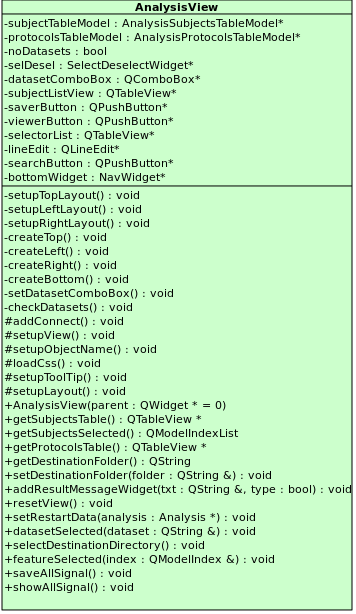
\includegraphics[width=0.5\linewidth]{./Content/Immagini/view/AnalysisView.png}
			\caption{Diagramma Classe AnalysisView: attributi e metodi}
			\label{cl_anaview}
\end{figure}
\paragraph{Descrizione \\}
Classe che rappresenta il widget per avviare un'analisi su un \dataset{}.
\paragraph{Utilizzo\\}
La classe implementerà i metodi virtuali puri della superclasse inoltre darà la possibilità all'utente di selezionare un \dataset{} sul quale effettuare un'analisi,selezionare quali \subject{} analizzare, scegliere quali risultati salvare per le Feature\g{} (per l'algoritmo, di default viene sia visualizzato, sia esportato), selezionare il path di dove salvare i risultati e infine far partire l'analisi.
\paragraph{Classi ereditate\\}
\begin{itemize}
\item Window::APanel.
\end{itemize}
%%%%%%%ATTRIBUTI%%%%%%%%%%%
\paragraph{\textcolor{black}{Attributi\\}}
\begin{itemize}
%subjectsTAbModel
\item\color{teal}\verb!-subjectsTableModel: AnalysisSubjectsTableModel*!
\color{black}
\subparagraph{Descrizione:} Rappresenta il model per la tabella contenente i \subject{}. 

%protTAbModel
\item\color{teal}\verb!-subjectsTableModel: AnalysisSubjectsTableModel*!
\color{black}
\subparagraph{Descrizione:} Rappresenta il model per la tabella contenente i \protocol{}. 

%noDataset
\item\color{teal}\verb!-noDatasets: bool!
\color{black}
\subparagraph{Descrizione:} Rappresenta il flag che vale true se non sono presenti \dataset{} all'interno dell'applicativo \project{}. 

%subList
\item\color{teal}\verb!- subjectsListView: QTableView*!
\color{black}
\subparagraph{Descrizione:} Rappresenta la tabella contenente la lista di \subject{}.

%selDesl
\item\color{teal}\verb!-selDesel: SelectDeselectWidget*!
\color{black}
\subparagraph{Descrizione:} Rappresenta il widget per selezionare/deselezionare tutti gli oggetti della lista.

%searchButton
\item\color{teal}\verb!-searchButton:QPushButton*!
\color{black}
\subparagraph{Descrizione:} Rappresenta il pulsante per la ricerca della cartella dove salvare i risultati dell'analisi.

%saverButton
\item\color{teal}\verb!-saverButton:QPushButton*!
\color{black}
\subparagraph{Descrizione:} Rappresenta il pulsante per il salvataggio dei risultati delle Feature Extractor\g{}.

%viewrButton
\item\color{teal}\verb!-viewerButton:QPushButton*!
\color{black}
\subparagraph{Descrizione:} Rappresenta il pulsante per la visualizzazione dei risultati delle Feature Extractor\g{} dopo averli calcolati.

%bottomWidget
\item\color{teal}\verb! bottomWidget:NavWidget*!
\color{black} 
\subparagraph{Descrizione:}
Puntatore al widget che rappresenta la parte bassa della finestra contentente i pulsanti per tornare indietro, la visualizzazione della guida interattiva, la possibilità di eliminare un \dataset{} e confermare successivamente l'operazione.
\end{itemize}
%%%%%%%%%  METODI
\paragraph{\textcolor{black}{Metodi\\}}
\begin{itemize}
%costruttore
\item\color{blue}\verb! + DatasetsView(parent : QWidget*=0)!
\subparagraph{Descrizione:}
\color{black}Costruttore per la classe DatasesView. 
\subparagraph{Argomenti:}
\begin{itemize}
\item \color{RoyalPurple}\verb!parent: QWidget*=0  !\\ Puntatore al QWidget padre di DatasetsView.
\end{itemize}

%setupLayout()
\item\color{blue}\verb! #setupLayout():void!
\color{black}
\subparagraph{Descrizione:} Metodo che implementa il contratto fornito dalla classe astratta \hyperref[speAPanel]{APanel}.
\subparagraph{Note:}
\begin{itemize}
\item questo metodo deve essere marcato virtuale;
\item questo metodo è stato ridefinito.
\end{itemize}
 
%createTop
\item\color{blue}\verb! -createTop():void!
\color{black}
\subparagraph{Descrizione:} Metodo che ha il compito di costruire la parte in alto del widget contenente l'elenco dei \subject e a lato lo spazio per visualizzare le informazioni.
 
%setDatasetCombo
\item\color{blue}\verb! -setDatasetComboBox():void!
\color{black}
\subparagraph{Descrizione:} Metodo che ha il compito di costruire la comboBox contenente i \dataset{} presenti all'interno dell'applicativo \project. 
 
%checkDataset
\item\color{blue}\verb! -checkDatasets():void!
\color{black}
\subparagraph{Descrizione:} Metodo che testa se sono presenti \dataset{} da mostrare.  
 
%createButtom
\item\color{blue}\verb! -createButtom():void!
\color{black}
\subparagraph{Descrizione:} Metodo che ha il compito di costruire la parte in basso del widget contenente il pulsante per ritornare alla pagine iniziale, e per l'accesso alla guida.

%setupTopLayout
\item\color{blue}\verb! -setupTopLayout():void!
\color{black}
\subparagraph{Descrizione:} Metodo che ha il compito di impostare la parte alta del layout della finestra.
  
%LOADCSS
\item\color{blue}\verb! #loadCss():void!
\color{black}
\subparagraph{Descrizione:} Metodo che implementa il contratto fornito dalla classe astratta \hyperref[spe]{APanel}.
 \subparagraph{Note}
 \begin{itemize}
  \item questo metodo deve essere marcato virtuale;
 \item questo metodo è stato ridefinito.
 \end{itemize}
 
%setupObjectName
\item\color{blue}\verb! #setupObjectName():void!
\color{black}
\subparagraph{Descrizione:} Metodo che implementa il contratto fornito dalla classe astratta \hyperref[speAPanel]{APanel}.
 \subparagraph{Note}
 \begin{itemize}
  \item questo deve essere marcato virtuale;
 \item questo metodo è stato ridefinito.
 \end{itemize}
 
%setupToolTip
\item\color{blue}\verb! #setupToolTip():void!
\color{black}
\subparagraph{Descrizione:} Metodo che implementa il contratto fornito dalla classe astratta \hyperref[speAPanel]{APanel}.
 \subparagraph{Note}
 \begin{itemize}
 \item questo metodo deve essere marcato virtuale;
 \item questo metodo è stato ridefinito.
 \end{itemize}
 
%addConnect
\item\color{blue}\verb! #addConnect():void!
\color{black}
\subparagraph{Descrizione:} Metodo che implementa il contratto fornito dalla classe astratta \hyperref[speAPanel]{APanel}.
 \subparagraph{Note}
 \begin{itemize}
 \item questo metodo deve essere marcato costante;
 \item questo metodo deve essere marcato virtuale;
 \item questo metodo è stato ridefinito.
 \end{itemize}
 
%setupView 
\item\color{blue}\verb! #setupView():void!
\color{black}
\subparagraph{Descrizione:} Metodo che implementa il contratto fornito dalla classe astratta \hyperref[speAPanel]{APanel}.
 \subparagraph{Note}
 \begin{itemize}
 \item questo metodo deve essere marcato virtuale;
 \item questo metodo è stato ridefinito.
 \end{itemize}

%getsubje
\item\color{blue}\verb! +getSubjectsTable():QTabelView*!
\color{black}
\subparagraph{Descrizione:} Metodo che ritorna il puntatore al campo dati \emph{subjectTableModel}.
 \subparagraph{Note}
 \begin{itemize}
 \item questo metodo deve essere marcato costante.
 \end{itemize}

%getproto
\item\color{blue}\verb! +getProtocolsTable():QTabelView*!
\color{black}
\subparagraph{Descrizione: }Metodo che ritorna il puntatore al campo dati \emph{protocolTableModel}.
 \subparagraph{Note}
 \begin{itemize}
 \item questo metodo deve essere marcato costante.
 \end{itemize} 
 
%getsubjeSelect
\item\color{blue}\verb! +getSubjectsSelected():QModelIndexList!
\color{black}
\subparagraph{Descrizione:} Metodo che ritorna i \subject{} selezionati nella tabella; ritorna una lista di indici.
 \subparagraph{Note}
 \begin{itemize}
 \item questo metodo deve essere marcato costante.
 \end{itemize} 
 
%getDestFolder
\item\color{blue}\verb! +getDestinationFolder(): QString!
\color{black}
\subparagraph{Descrizione: }Metodo che ritorna la cartella di destinazione selezionata.
 \subparagraph{Note}
 \begin{itemize}
 \item questo metodo deve essere marcato costante.
 \end{itemize} 
 
%setDestFolder
\item\color{blue}\verb! +setDestinationFolder(folder : const QString&): void!
\color{black}
\subparagraph{Descrizione:} Metodo che ritorna la cartella di destinazione selezionata.
 \subparagraph{Argomenti:}
 \begin{itemize}
 \item \color{RoyalPurple} \verb! folder:const QString& ! \\Rappresenta il path della cartella di destinazione.
 \end{itemize}  
 
%addResultMessag
\item \color{blue} \verb! + addResultMessageWidget(txt: const QString&, type: bool):void! 
\color{black}
\subparagraph{Descrizione:} Metodo che ha il compito di aggiungere il messaggio di risultato per avvenuta operazione o meno a seconda del valore del secondo parametro passato.
\subparagraph{Argomenti:}
\begin{itemize}
\item \color{RoyalPurple} \verb! txt: const QString& ! \\Rappresenta il testo da mostrare all'utente all'interno del widget;
\item \color{RoyalPurple} \verb!type : bool ! \\ Vale true se il messaggio è un messaggio di successo, false se il messaggio è di errore.
\end{itemize}
\subparagraph{Note:}
\begin{itemize}
\item il metodo deve essere marcato virtuale.
\end{itemize} 

%resetView
\item\color{blue}\verb! +resetView(): void!
\color{black}
\subparagraph{Descrizione:} Metodo che reimposta tutti i campi della view.

%resetView
\item\color{blue}\verb! +setRestartData(analysis: Analysis*): void!
\color{black}
\subparagraph{Descrizione:} Metodo che imposta la view con i dati riguardanti l'analisi da far ripartire
\subparagraph{Argomenti:}
\begin{itemize}
\item \color{RoyalPurple} \verb! analysis: Analysis*! \\ Rappresenta l'analisi da far ripartire.
\end{itemize}
%%%%%%%%%%% signals
%featsSelected
\item\color{blue}\verb! +featureSelected(index:const QModelIndex&) :void! (signal)
\color{black} 
\subparagraph{Descrizione:}
Signal\g{} emesso quando l'utente seleziona una Feature\g{}.
\subparagraph{Attributi:}
\begin{itemize}
\item \color{RoyalPurple}\verb! index: const QModelIndex& ! \\ rappresenta l'indice della Feature\g{} selezionato.
\end{itemize}

%datasetSelected
\item\color{blue}\verb! +datasetSelected(dataset:const QString&) : void! (signal)
\color{black} 
\subparagraph{Descrizione:}
Signal\g{} emesso quando l'utente seleziona una Feature\g{}.
\subparagraph{Attributi:}
\begin{itemize}
\item \color{RoyalPurple}\verb! dataset: const QString& ! \\ rappresenta il nome del \dataset{} selezionato.
\end{itemize}

%selectDEstiFolder
\item\color{blue}\verb! +selectDestinationDirectory():void! (signal)
\color{black} 
\subparagraph{Descrizione:}
Signal\g{} emesso quando l'utente preme il pulsante per la ricerca della cartella in cui salvare i risultati.

%saveAll
\item\color{blue}\verb! +saveAllSignal() :void! (signal)
\color{black} 
\subparagraph{Descrizione:}
Signal\g{} emesso quando l'utente preme il pulsante per salvare o non salvare tutto.

%showAll
\item\color{blue}\verb! +showAllSignal() :void! (signal)
\color{black} 
\subparagraph{Descrizione:}
Signal\g{} emesso quando l'utente preme il pulsante per visualizzare o non visualizzare tutto.
\end{itemize}
\pagebreak
\color{black}
%%%%%%%%%%%%%%%%%%%%%%%%
%	DETAILED	
%%%%%%%%%%%%%%%%%
\subsubsection{DetailedResult (class)}
\label{spedetRe}
\begin{figure}[!h]
\centering
			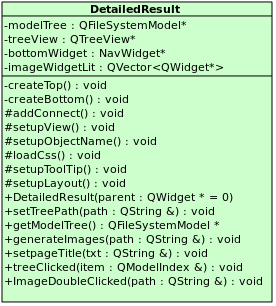
\includegraphics[width=0.5\linewidth]{./Content/Immagini/view/DetailedResult.png}
			\caption{Diagramma Classe DetailedResult: attributi e metodi}
			\label{cl_detRes}
\end{figure}
\paragraph{Descrizione \\}
Classe che rappresenta il widget per la visualizzazione di tutti i gruppi di \subject{} presenti all'interno di \project.
\paragraph{Utilizzo\\}
La classe implementerà i metodi virtuali puri della superclasse inoltre darà la possibilità all'utente di visualizzare l'elenco di tutti i gruppi di \subject{} fino a quel momento creati e memorizzati dentro a \project. Selezionando un gruppo, sarà possibile visualizzare le informazioni relative a quel gruppo, come per esempio i \subject{} contenuti al suo interno.
\paragraph{Classi ereditate\\}
\begin{itemize}
\item Window::APanel.
\end{itemize}
%%%%%%%ATTRIBUTI%%%%%%%%%%%
\paragraph{\textcolor{black}{Attributi\\}}
\begin{itemize}
%treeView
\item\color{teal}\verb!-treeView: QTreeView*!
\color{black}
\subparagraph{Descrizione:}
Rappresenta l'albero dei risultati di un'analisi. L'albero è ordinabile per l'elenco dei \subject{} su cui è stata effettuata l'analisi oppure per \protocol{} presenti nel \dataset{} su cui è stata eseguita l'analisi.

%modeltree
\item\color{teal}\verb!-modelTree: QFileSystemModel* !
\color{black}
\subparagraph{Descrizione:}
 Rappresenta il modello per l'albero dei risultati delle analisi.

%imageWidgetLit
\item\color{teal}\verb!-imageWidgetLit: QVector<QWidget*> !
\color{black}
\subparagraph{Descrizione:} Rappresenta il vettore contenenente i widget delle immagini.

%bottomWidget
\item\color{teal}\verb! bottomWidget:NavWidget*!
\color{black} 
\subparagraph{Descrizione:}
Puntatore al widget che rappresenta la parte bassa della finestra contentente i pulsanti per tornare indietro,e la visualizzazione della guida interattiva.
\end{itemize}
%%%%%%%%%  METODI
\paragraph{\textcolor{black}{Metodi\\}}
\begin{itemize}
%costruttore
\item\color{blue}\verb! + DetailedResult(parent : QWidget*=0)!
\color{black}
\subparagraph{Descrizione:} Costruttore per la classe DetailedResult. 
\subparagraph{Argomenti:}
\begin{itemize}
\item \color{RoyalPurple}\verb!parent: QWidget*=0 ! \\ Puntatore al QWidget padre di DetailedResult.
\end{itemize}

%setupLayout()
\item\color{blue}\verb! #setupLayout():void!
\color{black}
\subparagraph{Descrizione:} Metodo che implementa il contratto fornito dalla classe astratta \hyperref[speAPanel]{APanel}.
\subparagraph{Note:}
\begin{itemize}
\item questo metodo deve essere marcato virtuale;
\item questo metodo è stato ridefinito.
\end{itemize}
 
%createTop
\item\color{blue}\verb! -createTop():void!
\color{black}
\subparagraph{Descrizione:} Metodo che ha il compito di costruire la parte in alto del widget contenente l'elenco dei \subject e a lato lo spazio per visualizzare le informazioni.
 
%createButtom
\item\color{blue}\verb! -createButtom():void!
\color{black}
\subparagraph{Descrizione:} Metodo che ha il compito di costruire la parte in basso del widget contenente il pulsante per ritornare alla pagine iniziale, e per l'accesso alla guida.

%setupTopLayout
\item\color{blue}\verb! -setupTopLayout():void!
\color{black}
\subparagraph{Descrizione:} Metodo che ha il compito di impostare la parte alta del layout della finestra.
  
%LOADCSS
\item\color{blue}\verb! #loadCss():void!
\color{black}
\subparagraph{Descrizione:} Metodo che implementa il contratto fornito dalla classe astratta \hyperref[speAPanel]{APanel}.
 \subparagraph{Note}
 \begin{itemize}
  \item questo metododeve essere marcato virtuale;
 \item questo metodo è stato ridefinito.
 \end{itemize}
 
%setupObjectName
\item\color{blue}\verb! #setupObjectName():void!
\color{black}
\subparagraph{Descrizione:} Metodo che implementa il contratto fornito dalla classe astratta \hyperref[speAPanel]{APanel}.
 \subparagraph{Note}
 \begin{itemize}
  \item questo deve essere marcato virtuale;
 \item questo metodo è stato ridefinito.
 \end{itemize}
 
%setupToolTip
\item\color{blue}\verb! #setupToolTip():void!
\color{black}
\subparagraph{Descrizione:} Metodo che implementa il contratto fornito dalla classe astratta \hyperref[speAPanel]{APanel}.
 \subparagraph{Note}
 \begin{itemize}
 \item questo metodo deve essere marcato virtuale;
 \item questo metodo è stato ridefinito.
 \end{itemize}
 
%addConnect
\item\color{blue}\verb! #addConnect():void!
\color{black}
\subparagraph{Descrizione:} Metodo che implementa il contratto fornito dalla classe astratta \hyperref[speAPanel]{APanel}.
 \subparagraph{Note}
 \begin{itemize}
 \item questo metodo deve essere marcato costante;
 \item questo metodo deve essere marcato virtuale;
 \item questo metodo è stato ridefinito.
 \end{itemize}
 
%setupView
\item\color{blue}\verb! #setupView():void!
\color{black}
\subparagraph{Descrizione:} Metodo che implementa il contratto fornito dalla classe astratta \hyperref[speAPanel]{APanel}.
 \subparagraph{Note}
 \begin{itemize}
 \item questo metodo deve essere marcato virtuale;
 \item questo metodo è stato ridefinito.
 \end{itemize}
 
%setTreePath
\item\color{blue}\verb! +setTreePath(path: const QString&): void!
\color{black}
\subparagraph{Descrizione:} Metodo che imposta il path dell'albero da visualizzare
\subparagraph{Argomenti:}
\begin{itemize}
\item \color{RoyalPurple} \verb!path: const QString& ! \\ Rappresenta il path dell'albero.
\end{itemize}

%generateImages
\item\color{blue}\verb! +generateImages(path: const QString&): void!
\color{black}
\subparagraph{Descrizione:} Metodo che genera le immagini raggiungibili dal valore contenuto nel parametro
\subparagraph{Argomenti:}
\begin{itemize}
\item \color{RoyalPurple} \verb!path: const QString& ! \\ Rappresenta il path delle immagini da visualizzare.
\end{itemize}
 
 %setPageTitle
\item\color{blue}\verb! +setpageTitle(txt: const QString&): void!
\color{black}
\subparagraph{Descrizione:} Metodo che imposta il titolo nella parte alta della pagina.
\subparagraph{Argomenti:}
\begin{itemize}
\item \color{RoyalPurple} \verb! txt: const QString& ! \\ Rappresenta il testo da impostare come titolo.
\end{itemize}
 
%getModelTree
\item\color{blue}\verb! +getModelTree(): QFileSystemModel*!
\color{black}
\subparagraph{Descrizione:} Metodo che ritorna il campo dati \emph{modelTree}.
%%%%%%%%%%%%% signals
%treeclicked
\item\color{blue}\verb! + treeClicked(item:const QModelIndex&) : void! (signal)
\color{black} 
\subparagraph{Descrizione:} 
Signal\g{} emesso quando l'utente seleziona un elemento dall'albero.
\subparagraph{Attributi:}
\begin{itemize}
\item \color{RoyalPurple}\verb! item: const QModelIndex& ! \\ Rappresenta l'indice nell'albero selezionato.
\end{itemize}

%treeclicked
\item\color{blue}\verb!+ imageDoubleClicked(path:const QString&) : void! (signal)
\color{black} 
\subparagraph{Descrizione:} 
Signal\g{} emesso quando l'utente fa un doppio click sull'immagine visualizzata.
\subparagraph{Attributi:}
\begin{itemize}
\item \color{RoyalPurple}\verb! path: const QString& ! \\ Rappresenta il path relativo all'immagine.
\end{itemize}
 
\end{itemize}
\pagebreak
\color{black}
%%%%%%%%%%%%%%%
% RESULTSVIEW
%%%%%%%%%%%%%%
\subsubsection{ResultsView (class)}
\label{speResV}
\begin{figure}[!h]
\centering
			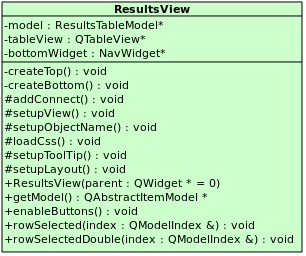
\includegraphics[width=0.45\linewidth]{./Content/Immagini/view/ResultsView.png}
			\caption{Diagramma Classe ResultsView: attributi e metodi}
			\label{cl_ResV}
\end{figure}
\paragraph{Descrizione \\}
Classe che rappresenta il widget per la visualizzazione di tutte le analisi effettuate contenute dentro a \project{}.Contiene sia le analisi complete, effettuate con successo sia quelle interrotte che quelle incomplete.
\paragraph{Utilizzo\\}
La classe implementerà i metodi virtuali puri della superclasse inoltre darà la possibilità all'utente di visualizzare l'elenco di tutte le analisi effettuate, e di aprire una nuova finestra per vedere nel dettaglio i risultati di una specifica analisi.
\paragraph{Classi ereditate\\}
\begin{itemize}
\item Window::APanel.
\end{itemize}
%%%%%%%ATTRIBUTI%%%%%%%%%%%
\paragraph{\textcolor{black}{Attributi\\}}
\begin{itemize}
%model
\item\color{teal}\verb!-model: ResultsTableModel*!
\color{black}
\subparagraph{Descrizione: } Rappresenta il modello per la tabella dei risultati delle analisi effettuate.

%tabelView
\item\color{teal}\verb!-tableView: QTableView*!
\color{black}
\subparagraph{Descrizione: }  
Contiene la lista di tutte le analisi effettuate anche se non complete (non eseguite su tutti i \subject del \dataset{}) e interrotte.

%bottomWidget
\item\color{teal}\verb! bottomWidget:NavWidget*!
\color{black} 
\subparagraph{Descrizione:}
 Puntatore al widget che rappresenta la parte bassa della finestra contentente i pulsanti per tornare indietro,e la visualizzazione della guida interattiva.
\end{itemize}
%%%%%%%%%  METODI
\paragraph{\textcolor{black}{Metodi\\}}
\begin{itemize}
%costruttore
\item\color{blue}\verb! + ResultsView(parent : QWidget*=0)!
\color{black}
\subparagraph{Descrizione:} Costruttore per la classe ResultsView. 
\subparagraph{Argomenti:}
\begin{itemize}
\item \color{RoyalPurple}\verb!parent: QWidget*=0  !\\ Puntatore al QWidget padre di ResultsView.
\end{itemize}

%setupLayout()
\item\color{blue}\verb! #setupLayout():void!
\color{black} 
\subparagraph{Descrizione:} Metodo che implementa il contratto fornito dalla classe astratta \hyperref[speAPanel]{APanel}.
\subparagraph{Note}
\begin{itemize}
\item questo metodo deve essere marcato virtuale;
\item questo metodo è stato ridefinito.
\end{itemize}
 
%createTop
\item\color{blue}\verb! -createTop():void!
\color{black}
\subparagraph{Descrizione:} Metodo che ha il compito di costruire la parte in alto del widget contenente l'elenco dei \subject e a lato lo spazio per visualizzare le informazioni.
 
%createButtom
\item\color{blue}\verb! -createButtom():void!
\color{black}
\subparagraph{Descrizione:} Metodo che ha il compito di costruire la parte in basso del widget contenente il pulsante per ritornare alla pagine iniziale, e per l'accesso alla guida.

%setupTopLayout
\item\color{blue}\verb! -setupTopLayout():void!
\color{black}
\subparagraph{Descrizione:} Metodo che ha il compito di impostare la parte alta del layout della finestra.
  
%LOADCSS
\item\color{blue}\verb! #loadCss():void!
\color{black}
\subparagraph{Descrizione:} Metodo che implementa il contratto fornito dalla classe astratta \hyperref[speAPanel]{APanel}.
 \subparagraph{Note}
 \begin{itemize}
  \item questo metododeve essere marcato virtuale;
 \item questo metodo è stato ridefinito.
 \end{itemize}
 
%setupObjectName
\item\color{blue}\verb! #setupObjectName():void!

\color{black}
\subparagraph{Descrizione:} Metodo che implementa il contratto fornito dalla classe astratta \hyperref[speAPanel]{APanel}.
 \subparagraph{Note}
 \begin{itemize}
  \item questo deve essere marcato virtuale;
 \item questo metodo è stato ridefinito.
 \end{itemize}
 
%setupToolTip
\item\color{blue}\verb! #setupToolTip():void!

\color{black}
\subparagraph{Descrizione:} Metodo che implementa il contratto fornito dalla classe astratta \hyperref[speAPanel]{APanel}.
 \subparagraph{Note}
 \begin{itemize}
 \item questo metodo deve essere marcato virtuale;
 \item questo metodo è stato ridefinito.
 \end{itemize}
 
%addConnect
\item\color{blue}\verb! #addConnect():void!

\color{black}
\subparagraph{Descrizione:} Metodo che implementa il contratto fornito dalla classe astratta \hyperref[speAPanel]{APanel}.
 \subparagraph{Note}
 \begin{itemize}
 \item questo metodo deve essere marcato costante;
 \item questo metodo deve essere marcato virtuale;
 \item questo metodo è stato ridefinito.
 \end{itemize}
 
%setupView
\item\color{blue}\verb! #setupView():void!
\color{black}
\subparagraph{Descrizione:} Metodo che implementa il contratto fornito dalla classe astratta \hyperref[speAPanel]{APanel}.
 \subparagraph{Note}
 \begin{itemize}
 \item questo metodo deve essere marcato virtuale;
 \item questo metodo è stato ridefinito.
 \end{itemize}
\color{black}

%enableButtons
\item\color{blue}\verb! + enableButtons():void!
\color{black}
\subparagraph{Descrizione:} Metodo che ha il compito di abilitare i pulsanti presenti nella view.
\color{black}
%getModel
\item\color{blue}\verb! +getModelTree(): QFileSystemModel*!
\color{black}
\subparagraph{Descrizione:} Metodo che ritorna il campo dati \emph{model}.
\subparagraph{Note:}
\begin{itemize}
\item il metodo deve essere marcato come costante;
\end{itemize}

%%%%%%%%%%%%% signals
%rowSelected
\item\color{blue}\verb! + rowSelected(index :const QModelIndex&) : void! (signal)
\color{black} 
\subparagraph{Descrizione:} 
Signal\g{} emesso quando l'utente seleziona un elemento dalla tabella.
\subparagraph{Attributi:}
\begin{itemize}
\item \color{RoyalPurple}\verb! index: const QModelIndex& ! \\ Rappresenta l'indice della tabella selezionato.
\end{itemize}

%rowSelectDoubl
\item\color{blue}\verb! + rowSelected(index :const QModelIndex&) : void! (signal)
\color{black} 
\subparagraph{Descrizione:} 
Signal\g{} emesso quando l'utente fa il doppio click su un elemento dalla tabella.
\subparagraph{Attributi:}
\begin{itemize}
\item \color{RoyalPurple}\verb! index: const QModelIndex& ! \\ Rappresenta l'indice della tabella selezionato.
\end{itemize}

\end{itemize}
\color{black}